\chapter{Methodik und Versuchsaufbau}
\label{ch:chapter04}

In diesem Kapitel wird die methodische Vorgehensweise der Arbeit detailliert erläutert. 
Ziel ist es, eine reproduzierbare und nachvollziehbare Grundlage für die experimentelle Evaluation zu schaffen. 
Diese Grundlage kann eventuell in Zukunft auch in anderen Projekten wiederverwendet werden.

\section{Auswahl der Microbenchmarks} 
\label{sec:auswahl-microbenchmarks}

Die Auswahl geeigneter Microbenchmarks ist entscheidend für die Aussagekraft der Ergebnisse. 
Sie müssen typische Interaktionsmuster von \ac{FaaS}-Instanzen repräsentieren. 
In Anlehnung an die Arbeit von Eder et al.~\cite{10254754} werden fünf Szenarien verwendet (siehe Abbildung~\ref{fig:chapter02:aws_lambda_use_cases}), 
die auf einer umfassenden Analyse der häufigsten Anwendungsfälle von AWS Lambda durch Winzinger et al.~\cite{Winzinger2021DataFlow} 
basieren.


Alle fünf Benchmarks werden in den drei zu untersuchenden Sprachen Java, Python und NodeJS implementiert. 
Die Funktionalität ist dabei jeweils identisch. Der Kern der Funktion besteht ausschließlich aus dem Aufruf der 
entsprechenden AWS-SDK-Methode, um den Overhead der Geschäftslogik minimal zu halten und den Instrumentierungsoverhead 
möglichst gut zu isolieren.

\section{Konfiguration und Entwicklung der Funktionen}
\label{sec:entwicklung-funktionen}
\paragraph{Entwicklung der Funktionen}
Für jede der drei Sprachen und jeden der fünf Microbenchmarks wurde eine eigene Lambda-Funktion erstellt. 
Alle Funktionen nutzen die offiziellen AWS SDKs. 
Die Funktionen basieren auf der Arbeit von Eder et al \cite{10254754} und wurden für Zwecke der Konsistenz weitgehend repliziert. 
Alle Funktionen verwenden dieselbe, minimal notwendige Logik. Entgegennahme eines Events, Ausführen der Zieloperation und Rückgabe einer 
einfachen Bestätigung. 
Um den ökologischen Fußabdruck dieser Arbeit zu reduzieren und Ressourcen zu schonen, wurde ähnlich wie bei der Arbeit von Eder et al \cite{10254754} 
auf den Abdruck von Quellcode, Konfigurationsdateien und weiterführenden technischen Materialien im Anhang verzichtet. 
Alle relevanten Implementierungen sowie deren vollständige Dokumentation sind öffentlich in einem GitHub-Repository verfügbar und 
können unter folgender Adresse eingesehen werden: [www.github.com/justaksi7/kommt-noch]. Dies gewährleistet nicht nur Nachhaltigkeit, 
sondern auch Transparenz und Reproduzierbarkeit der erzielten Ergebnisse.

\paragraph{Konfiguration der AWS Lambda-Umgebung}
Um eine hohe Vergleichbarkeit der Messungen zu gewährleisten, werden alle Funktionen mit identischen, kontrollierten 
Parametern betrieben. Die Konfiguration orientiert sich an typischen Produktionseinstellungen und wird über die AWS Management Console 
sowie Infrastructure-as-Code (AWS SAM) festgelegt.

Tabelle~\ref{tab:konfiguration} fasst die konstant gehaltenen Konfigurationsparameter zusammen.

\begin{table}[H]
\centering
\caption{Konstante Konfigurationsparameter der Lambda-Funktionen}
\label{tab:konfiguration}
\begin{tabular}{|p{3cm}|p{3cm}|p{5.5cm}|}
\hline
\textbf{Parameter} & \textbf{Wert} & \textbf{Begründung} \\
\hline
Region & \texttt{Frankfurt (eu-central-1)} & Minimierung von Netzwerklatenz-Varianz durch einheitliche Region. \\
\hline
Speicher (Memory) & 1024 MB & Ausreichend für den Funktionsumfang. \\
\hline
Ephemeraler Speicher & 512 MB & Standardwert, für die Funktionen ausreichend. \\
\hline
Timeout & 15 Sekunden & Ausreichend für alle Benchmarks (auch langsamste Kombination). \\
\hline
Reservierte Konkurrenz & 200 & Begrenzung der parallelen Ausführungen, um kontrollierte Last zu erzeugen und Überlastung zu vermeiden. \\
\hline
Laufzeit (Runtime Environment) & Java 21, Python 3.13, NodeJS 22.x & Aktuelle, von \ac{ADOT}-Lambda-Layers unterstützte Versionen der Sprachen. \\
\hline
IAM-Rolle &  Rolle mit minimalen Berechtigungen & Erlaubt nur die notwendigen Aktionen: \texttt{lambda:InvokeFunction} für Benchmark 1 
und \texttt{dynamodb:GetItem} / \texttt{PutItem} für Benchmarks 4 / 5, sowie das Schreiben von Logs auf CloudWatch. \\
\hline
\end{tabular}
\end{table}

Die reservierte Konkurrenz von 200 wurde gewählt, um eine definierte maximale Parallelität zu haben. Dies verhindert, 
dass AWS Lambda unbegrenzt skaliert und möglicherweise die Messergebnisse durch unterschiedliches Skalierungsverhalten bei den 
verschiedenen Funktionen verfälscht.

Für die Implementierung wurden ausschließlich die offiziellen AWS SDKs und Standardbibliotheken für HTTP-Requests für alle 3 
Sprachen verwendet. Für jeden AWS-Dienst (Lambda, DynamoDB usw.) gibt es ein separates SDK-Modul in den jeweiligen Sprachen 
und für jede Sprache und Region gibt es eine dedizierte ADOT-Lambda-Layer, die über den \ac{ARN} referenziert wird.
Eine detailierte Übersicht über die \textbf{importierten} \footnote{Bibliotheken und SDKs, 
die in den jeweiligen Sprachen bereits integriert sind (wie z. B. fetch in NodeJS) wurden hier nicht aufgeführt. 
Die vollständigen Implementierungen sind im GitHub-Repository unter \url{https://github.com/justaksi7/kommt-noch} verfügbar.} 
Bibliotheken und SDKs für die Implementierungen ist in 
Tabellen~\ref{tab:java-libraries}, \ref{tab:python-libraries} und \ref{tab:nodejs-libraries} dargestellt.

\begin{table}[H]
\centering
\caption{Verwendete Bibliotheken und SDKs für Java}
\label{tab:java-libraries}
\begin{tabular}{|p{3.5cm}|p{9cm}|}
\hline
\textbf{Benchmark} & \textbf{Verwendete Bibliotheken / SDKs} \\
\hline
1. Lambda-Aufruf & AWS Lambda Runtime v2.41.34 (Context, RequestHandler), AWS SDK v2.41.34 für Lambda (LambdaClient, InvokeRequest, InvocationType, SdkBytes) \\
\hline
2. HTTP GET & AWS Lambda Runtime v2.41.34, Java HTTP Client (java.net.http.HttpClient, HttpRequest, HttpResponse) \\
\hline
3. HTTP POST & AWS Lambda Runtime v2.41.34, Java HTTP Client, Gson v2.13.2 (JSON-Verarbeitung) \\
\hline
4. DynamoDB Read & AWS Lambda Runtime v2.41.34, AWS SDK v2.41.34 für DynamoDB (DynamoDbClient, AttributeValue, GetItemRequest, GetItemResponse) \\
\hline
5. DynamoDB Write & AWS Lambda Runtime v2.41.34, AWS SDK v2.41.34 für DynamoDB (PutItemRequest, DynamoDbException), java.util.UUID \\
\hline
\end{tabular}
\end{table}

\begin{table}[H]
\centering
\caption{Verwendete Bibliotheken und Module für Python}
\label{tab:python-libraries}
\begin{tabular}{|p{3.5cm}|p{9cm}|}
\hline
\textbf{Benchmark} & \textbf{Verwendete Bibliotheken / Module} \\
\hline
1. Lambda-Aufruf & boto3 (AWS SDK), json \\
\hline
2. HTTP GET & urllib3 \\
\hline
3. HTTP POST & urllib3, json \\
\hline
4. DynamoDB Read & boto3, json \\
\hline
5. DynamoDB Write & boto3, uuid, json \\
\hline
\end{tabular}
\end{table}

\begin{table}[H]
\centering
\caption{Verwendete Bibliotheken und Module für NodeJS}
\label{tab:nodejs-libraries}
\begin{tabular}{|p{3.5cm}|p{9cm}|}
\hline
\textbf{Benchmark} & \textbf{Verwendete Bibliotheken / Module} \\
\hline
1. Lambda-Aufruf & @aws-sdk/client-lambda (LambdaClient, InvokeCommand)\\
\hline
2. HTTP GET & Keine\\ 
\hline
3. HTTP POST & Keine\\ 
\hline
4. DynamoDB Read & @aws-sdk/client-dynamodb (DynamoDBClient, GetItemCommand)\\
\hline
5. DynamoDB Write & @aws-sdk/client-dynamodb (DynamoDBClient, PutItemCommand), crypto.randomUUID\\
\hline
\end{tabular}
\end{table}

Eine detaillierte Dokumentation der verwendeten Bibliotheken und SDKs ist besonders wichtig, da sie die Performance der Funktionen 
bei Java signifikant beeinflussen kann. Diese Beobachtung basiert auf der Erfahrung aus der vorliegenden Arbeit.

\section{Konfiguration der Infrastruktur für die Benchmarks}
\paragraph{Benchmark 1 - Aufgerufene Lambda-Funktion}
Die aufgerufene Lambda Funktion für Benchmark 1 wurde mit einer minimalen Konfiguration erstellt. Sie wurde asynchron mithilfe von Events 
aufgerufen, wobei die InvocationType auf \texttt{Event} gesetzt wurde. Das bedeutet, dass die aufrufende Funktion nicht auf die Antwort der 
aufgerufenen Funktion wartet, sondern sofort fortfährt. Die vollständige Konfiguration der aufgerufenen Lambda-Funktion ist in Tabelle~\ref{tab:aufgerufene-lambda-config} dargestellt.
\begin{table}[H]
\centering
\caption{Konfigurationsparameter der aufgerufenen Lambda-Funktion (Benchmark 1)}
\label{tab:aufgerufene-lambda-config}
\begin{tabular}{|p{4cm}|p{4.5cm}|}
\hline
\textbf{Parameter} & \textbf{Wert} \\
\hline
Region & Frankfurt (eu-central-1) \\
\hline
Speicher (Memory) & 128 MB \\
\hline
Ephemeraler Speicher & 512 MB \\
\hline
Timeout & Standard (3 Sekunden) \\
\hline
Reservierte Konkurrenz (Reserved Concurrency) & 200 \\
\hline
Laufzeit (Runtime Environment) & Node.js 22.x \\
\hline
IAM-Rolle & Standard-Lambda-Rolle (Standardausführung) \\
\hline
\end{tabular}
\end{table}
Die aufgerufene Lambda Funktion für Benchmark 1 wurde mit einer minimalen Konfiguration erstellt. Sie wurde asynchron mithilfe von Events 
aufgerufen, wobei die InvocationType auf \texttt{Event} gesetzt wurde. Das bedeutet, dass die aufrufende Funktion nicht auf die Antwort der 
aufgerufenen Funktion wartet, sondern sofort fortfährt. Das isoliert die Performance der aufrufenden Funktion.

\section{Instrumentierung mit OpenTelemetry (ADOT)}
\label{sec:instrumentierung}

Um den Tracing-Overhead zu messen, wurden die Lambda-Funktionen mit OpenTelemetry instrumentiert. Hierfür kam die AWS Distro for 
OpenTelemetry \ac{ADOT} zum Einsatz. ADOT bietet vorgefertigte Lambda-Layer für jede unterstützte Sprache, die alle notwendigen 
Abhängigkeiten (SDK, Collector, Exporters) enthalten. Um im Rahmen der Zeit- und Ressourcenbeschränkungen dieser Arbeit zu bleiben, 
wurde auf eine manuelle, Code-basierte Instrumentierung verzichtet. Stattdessen erfolgte die Instrumentierung, wie in der Arbeit von
Eder. et al \cite{10254754}, ausschließlich über die automatische Erfassung von Traces durch \ac{ADOT}.
Als Sampling-Strategie wurde \emph{Head Sampling} mit einer Rate von 100\,\% verwendet, d.~h. jeder Trace wurde vollständig aufgezeichnet. 
Die so instrumentierten Funktionen exportieren die Trace-Daten über den ADOT-Collector an \emph{AWS X-Ray}. 
X-Ray dient als Tracing-Backend und ermöglicht die spätere Überprüfung der Vollständigkeit der Traces. 
Die Integration wurde über die Umgebungsvariable \texttt{AWS\_LAMBDA\_EXEC\_WRAPPER} bzw. durch entsprechende Konfiguration in 
der \texttt{function.properties} der Lambda-Funktionen realisiert.

\section{Messgrößen und Berechnung des Overheads}
\label{sec:messgroessen}

Die zentralen Performance-Metriken wurden aus den von AWS bereitgestellten CloudWatch Logs extrahiert. Jede Lambda-Invocation 
erzeugt einen Logeintrag, der die folgenden Felder enthält:

\begin{itemize}
    \item \emph{\texttt{Duration}} (in ms): Die vom Handler gemessene Ausführungsdauer der Funktion. 
	Sie umfasst die Zeit von Beginn der Handler-Ausführung bis zu deren Ende.
    \item \emph{\texttt{Max Memory Used}} (in MB): Der maximale Arbeitsspeicher, der während der Ausführung benutzt wurde.
    \item \emph{\texttt{Init Duration}} (in ms): Die Dauer der Initialisierungsphase bei einem Kaltstart. Dieses Feld erscheint 
	nur im Logeintrag der Kaltstarts.
\end{itemize}

Zusätzlich wurde für die instrumentierten Funktionen die Anzahl der erzeugten Traces überprüft (durch Abfragen in der AWS X-Ray 
Konsole bzw. im CLI), um sicherzustellen, dass für jede Invocation tatsächlich ein Trace exportiert wurde.

Der relative prozentuale Overhead für eine Metrik \(M\) wurde wie folgt berechnet:

\begin{equation}
\text{Overhead}_{M} = \frac{M_{\text{mit OTel}} - M_{\text{ohne OTel}}}{M_{\text{ohne OTel}}} \times 100\%
\label{eq:overhead}
\end{equation}

Dabei bezeichnet \(M_{\text{mit OTel}}\) den gemessenen Wert der instrumentierten Version und \(M_{\text{ohne OTel}}\) 
den Wert der nicht instrumentierten Baseline. Für die Berechnung wurden jeweils die Mittelwerte über alle gültigen Messungen 
einer Kombination (Sprache, Benchmark, Instrumentierungsstatus) verwendet. Kaltstart- und Warmstartmessungen wurden separat 
betrachtet.

\section{Durchführung der Messungen}
\label{sec:durchfuehrung}

Die Messungen wurden in mehreren Phasen durchgeführt, um eine ausreichende statistische Basis zu schaffen und 
Störeinflüsse zu minimieren. Es wurden jeweils 10 Messvorgänge je 1.200 Aufrufe pro Kombination (Sprache, Benchmark, 
Instrumentierungsstatus) durchgeführt, was insgesamt 12.000 Aufrufe (jeweils ~10.000 Warmstarts und ~2.000 Kaltstarts) pro 
Kombination ergibt. Nach jedem Messvorgang wurden die Funktionen, wie bei der Arbeit von Eder et al. \cite{10254754} erneut deployed, 
um Kaltstarts zu erzwingen und eine Durchmischung der Ausführungsumgebungen zu gewährleisten. Das 
reduziert die Wahrscheinlichkeit, dass mehrere Aufrufe auf derselben physischen Maschine ausgeführt werden. 
\\Die Aufrufe wurden mit einem Python-Skript parallelisiert, 
um die reservierte Konkurrenz von 200 zu nutzen und eine realistische Last zu simulieren. Es wurde jedoch kaum eine Parallelität 
von 200 erreicht, da die Funktionen aufgrund der kurzen Ausführungszeiten schnell freigegeben wurden. Nur in einigen Fällen, 
insbesondere bei Java, kam es zu kurzzeitigen Spitzen von bis zu 200 parallelen Ausführungen bei den Kaltstarts. Die Parallelität sank 
unmittelbar nach einigen Aufrufen im Anschluss an die Kaltstarts wieder auf wenige parallele Aufrufe (15 bis 30). Dies gewährleistet, 
dass die Einschwingphase der Funktionen (\ac{JIT}-Optimierung bei Java und NodeJS und Bytecode-Optimierung bei Python) 
gut abgedeckt wird, da es genug Warmstarts nach den Optimierungen gab und ein stabiler Zustand erreicht wurde. Da mindestens 
2.000 Kaltstarts pro Kombination angestrebt wurden, wurden die Funktionen ergänzend zu den 10 Messvorgängen solange redeployed und 
aufgerufen, bis die gewünschte Anzahl an Kaltstarts erreicht wurde.

\paragraph{Berücksichtigung der Einschwingphase}
Da die Funktionen wegen \ac{JIT}-Compiler bei Java und NodeJS und Bytecode-Optimierung bei Python erst nach mehreren Durchläufen 
optimierten Code produzieren, wurden bei der Auswertung nicht nur die Mittelwerte, sondern auch die Mediane der Messergebnisse betrachtet. 
Die Mediane sind weniger anfällig für Ausreißer und geben einen besseren Einblick in die typische Performance nach der Einschwingphase~\cite{MedianVsMean}.

\section{Statistische Auswertung}
\label{sec:auswertung}

Um die in Kapitel~\ref{ch:chapter01} formulierten Forschungsfragen zu beantworten, wurden die folgenden Hypothesen aufgestellt. 
Dabei werden zwei grundsätzliche Fragestellungen adressiert - der Unterschied zwischen Messungen ohne Tracing und mit Tracing (H1) 
sowie die Abweichungen zwischen den einzelnen Programmiersprachen (H2).

\paragraph{H1 – Sprachspezifischer Overhead}
Der Effizienz-Overhead ohne Einsatz von OpenTelemetry ist geringer als der Overhead bei Verwendung von OpenTelemetry in einer bestimmten Programmiersprache \(s\). Formal ausgedrückt:
\[
H_0: \mu_{\text{ohne}} \ge \mu_s \quad \text{vs.} \quad H_1: \mu_{\text{ohne}} < \mu_s,
\]
wobei \(\mu_{\text{ohne}}\) den mittleren Wert der betrachteten Metrik (z.B. Laufzeit, Speicherverbrauch, Kaltstartdauer) ohne Instrumentierung und \(\mu_s\) den entsprechenden Wert mit Instrumentierung in Sprache \(s\) bezeichnet.

\paragraph{H2 – Sprachvergleiche}
Es besteht ein signifikanter Unterschied im Effizienz-Overhead zwischen zwei verschiedenen Programmiersprachen \(s_1\) und \(s_2\). Formal:
\[
H_0: \mu_{s_1} = \mu_{s_2} \quad \text{vs.} \quad H_1: \mu_{s_1} \neq \mu_{s_2}.
\]
In beiden Fällen wurde von unbekannter Varianz ausgegangen. Für das Signifikanzniveau wurde \(\alpha = 0{,}05\) festgelegt.

\subsection{Durchführung der statistischen Tests}

Zur Überprüfung der beiden Hypothesen wurden unterschiedliche statistische Verfahren eingesetzt, die den jeweiligen Datenstrukturen und Fragestellungen Rechnung tragen.

\paragraph{H1 – Vergleich mit und ohne Instrumentierung}
Für jede Programmiersprache \(s\) wurden die Messwerte der instrumentierten und der nicht-instrumentierten Funktion gegenüberstellt. 
Da es sich um gepaarte Messungen handelt (jeder Aufruf der instrumentierten Funktion entspricht einem Aufruf derselben Funktion 
ohne Instrumentierung unter identischen Bedingungen), wurde ein \emph{einseitiger Welch's t-Test}~\cite{WelchsTTest} durchgeführt.  
Das Signifikanzniveau wurde auf \(\alpha = 0{,}05\) festgelegt.

\paragraph{H2 – Vergleich zwischen verschiedenen Programmiersprachen}
Für den paarweisen Vergleich der Sprachen (Java vs. Python, Java vs. NodeJS, Python vs. NodeJS) lagen unabhängige Stichproben vor. 
Da die Stichprobenumfänge begrenzt sind (jeweils nur 1 Mittelwert pro Messung), kam ein nichtparametrisches 
\emph{Bootstrap-Hypothesentest}~\cite{Bootstrapping} zum Einsatz. Konkret wurde ein 
\emph{Perzentil-Bootstrap} mit \(R = 100.000\) Resamples durchgeführt. D. h. es wurden 100.000 Stichproben mit Zurücklegen 
für jede originale Stichprobe gezogen (100.000 Mal die Differenz der Mittelwerte zwischen der instrumentierten und 
nicht-instrumentierten Funktion für jede Sprache \(s\)). Anschließend wurden paarweise die p-Werte mittels Bootstrap-Hypothesentest 
berechnet. Dabei wurde verglichen, wie oft der Overhead der einen Sprache größer oder kleiner als der der anderen Sprache ist. Das 
Signifikanzniveau wurde ebenfalls auf \(\alpha = 0{,}05\) festgelegt.

\begin{itemize}
    \item \textbf{Visuelle Aufbereitung:} Die Ergebnisse werden mittels Boxplots visualisiert, um die Verteilung und Ausreißer 
	darzustellen. Zusätzlich werden Balkendiagramme für den direkten Vergleich der prozentualen Overheads verwendet.
    \item \textbf{Software:} Die statistische Auswertung erfolgt mit der Programmiersprache Python unter Verwendung der Bibliotheken \texttt{pandas}, \texttt{numpy}, \texttt{scipy.stats}, \texttt{statsmodels} und \texttt{matplotlib} / \texttt{seaborn} für die grafische Darstellung.
\end{itemize}

Die Ergebnisse dieser Auswertung werden in Kapitel~\ref{ch:ergebnisse} präsentiert und in Kapitel~\ref{ch:diskussion} diskutiert.

\begin{figure}[htbp]
 \centering
 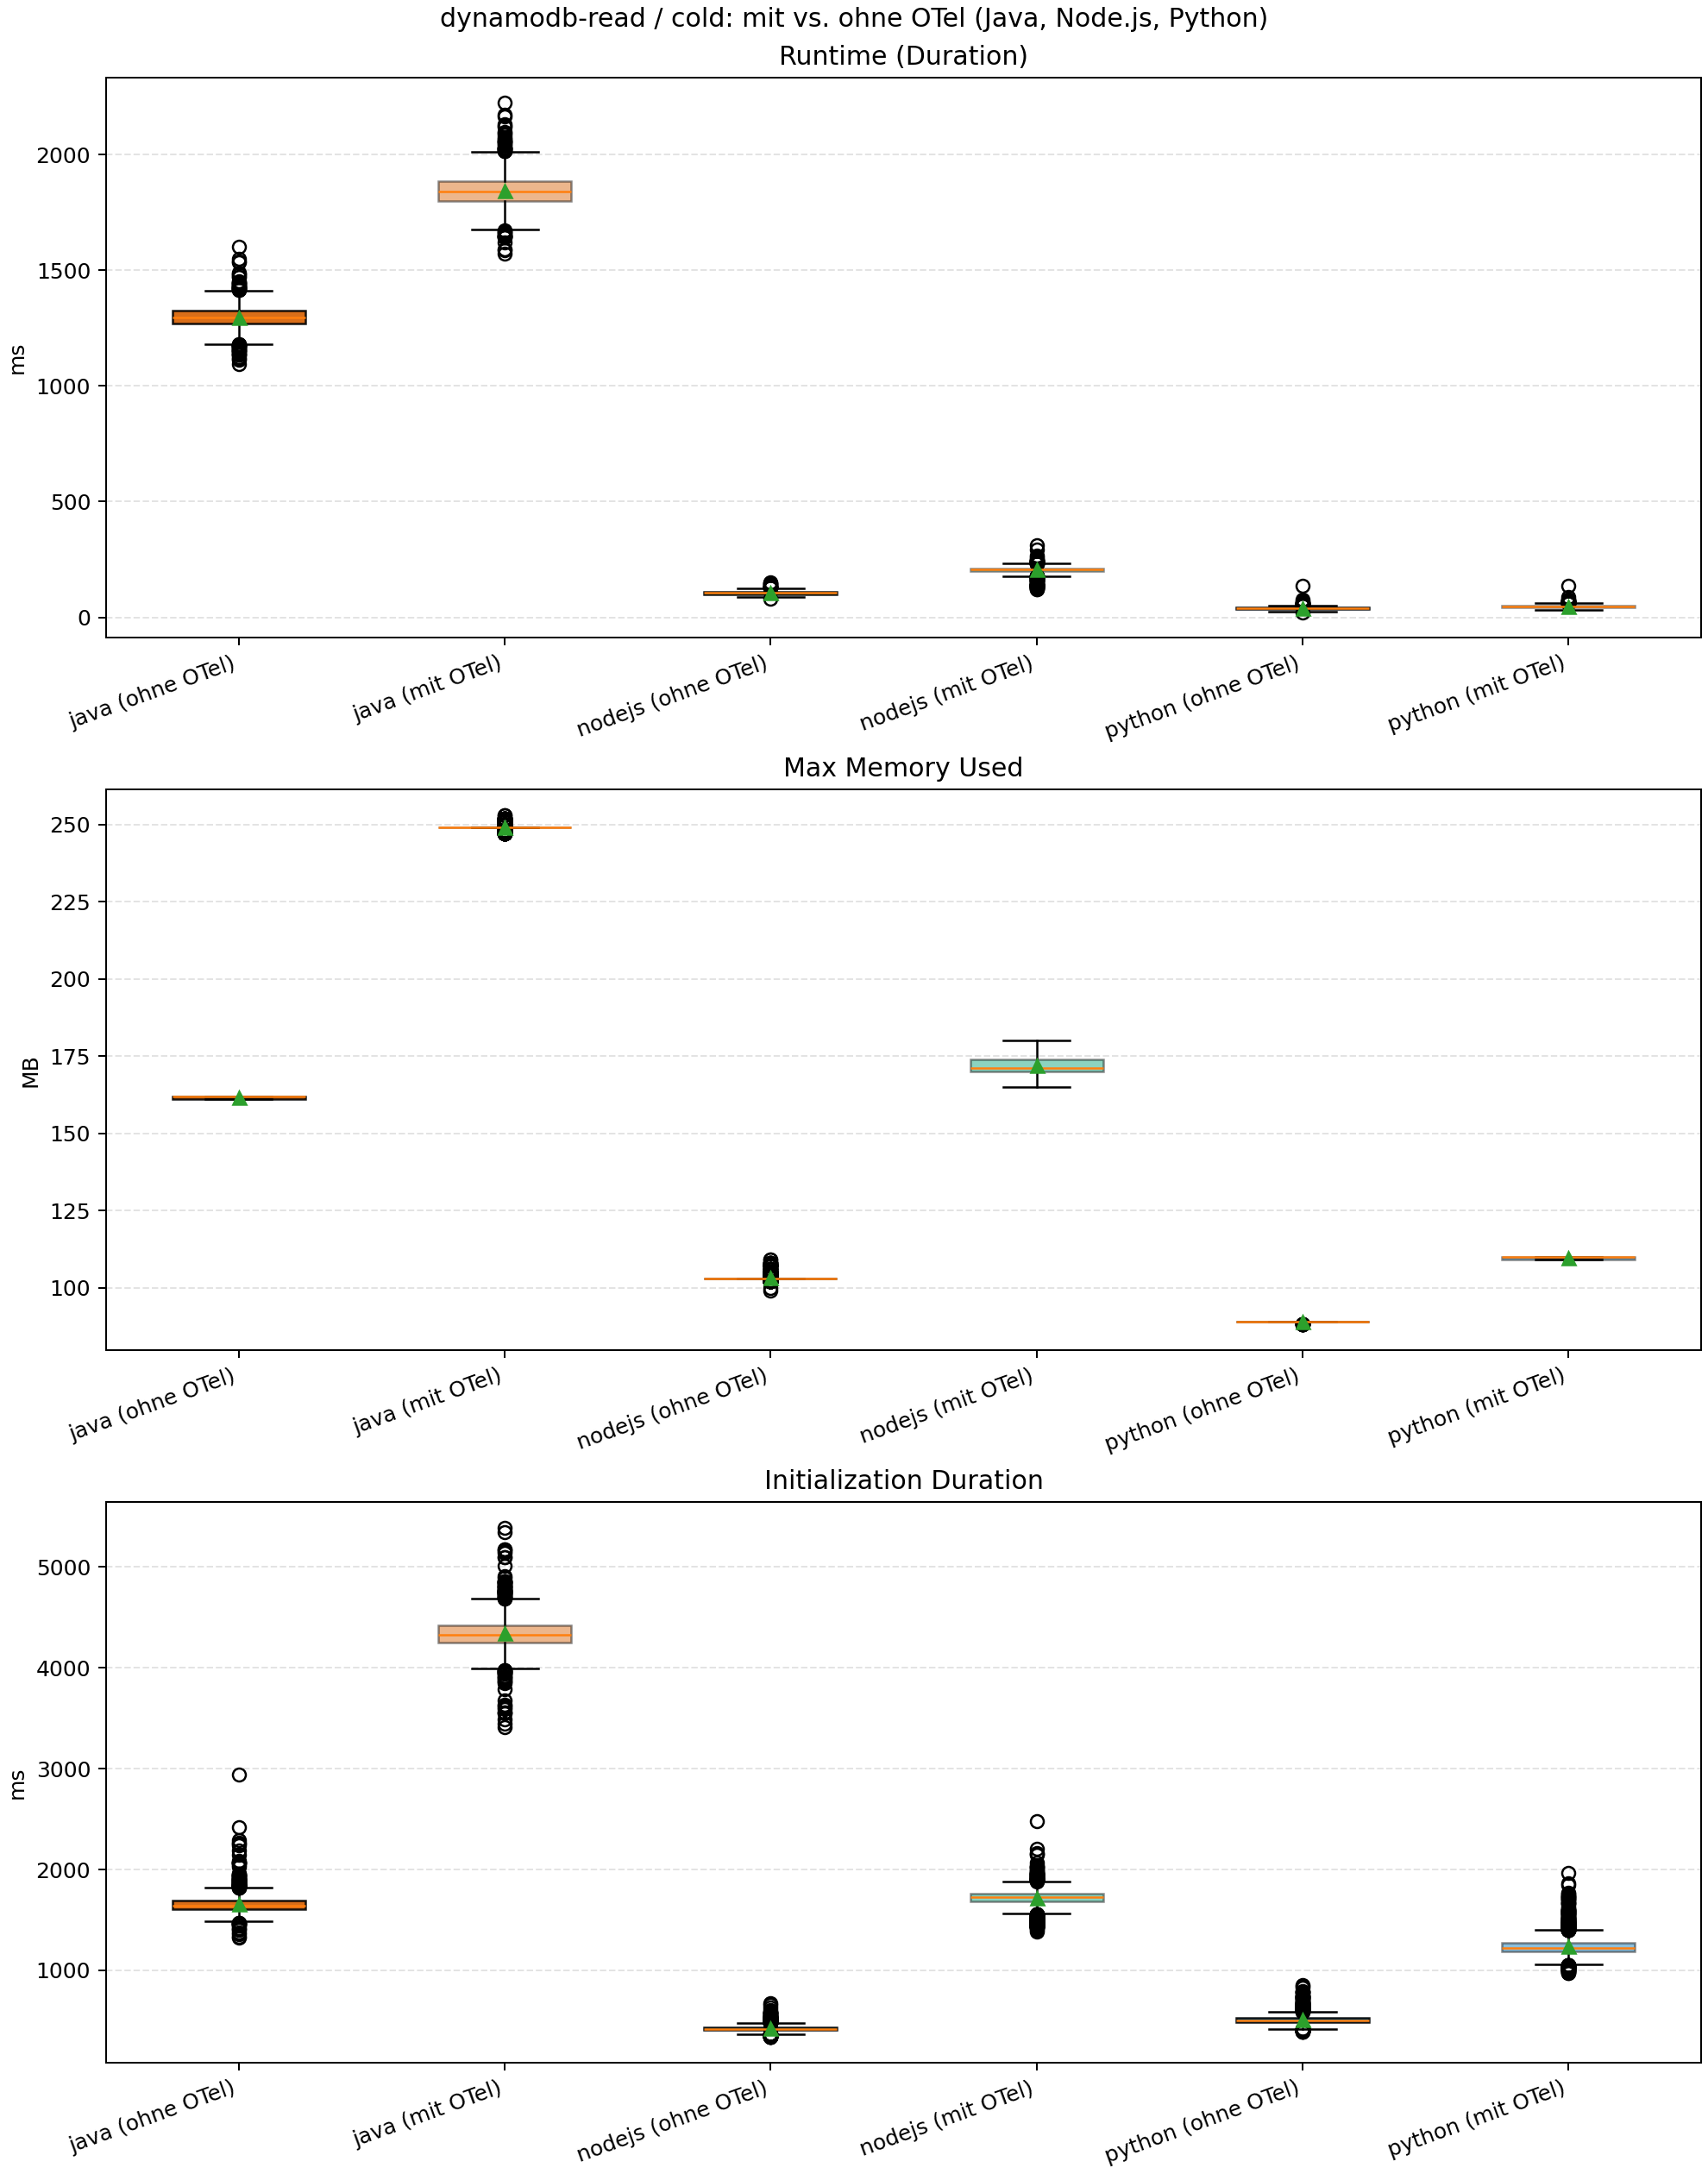
\includegraphics[width=1.0\textwidth]{gfx/examples/dynamodb-read-cold-otel-comparison.png}	
\end{figure}